En esta sección se detalla el diseño del sistema. Primero haremos una
descripción y justificación de las grandes decisiones arquitectónicas
tomadas, para luego hacer una descripción más detallada del sistema
entregado.

\subsection{Minilenguaje como DSL interna}
Finalmente la DSL se ha implementado por medio de una DSL~interna en
JRuby. Discutiremos las características de las DSL~internas y las
DSL~externas, así como la razón para elegir JRuby.
\subsubsection{DSL internas}
Definición, ventajas, inconvenientes, \ldots{}
\subsubsection{DSL externas}
Definición, ventajas, inconvenientes, \ldots{}
% JavaCC, ANTLR
\subsubsection{¿Por qué DSL interna?}
\subsubsection{Ruby y JRuby}
\subsubsection{Sintaxis}
\subsubsection{Ejemplos}

\subsubsection{Inyección código malicioso}
Se ha empleado una sandbox, Java Security Architecture, \ldots{}
\subsubsection{Timeouts}
\subsubsection{Manipulación estado intérprete}
\label{interpreter_state_manipulation}

\subsection{Servicio sigue estilo arquitectónico REST}
REST\footnote{\emph{Representational state transfer}} es un estilo de
arquitectura software empleado en sistemas distribuidos como la
\emph{World Wide Web}, de ahora en adelante \emph{WWW}.

REST fue desarrollado por Roy Fielding entre otros al mismo tiempo que
se desarrollaba la versión 1.1 del protocolo HTTP. Aun así REST se
puede emplear con otros protocolos si proporcionan mecanismos
adecuados para la transferencia de representación.

El objetivo de la WWW era constituir un espacio común de información
en el que máquinas y usuarios se puedan comunicar.  Los usuarios de
este sistema estarían por todo el mundo, en varias universidades e
institutos de investigación conectados a través de Internet. Las
máquinas así conectadas serían de carácter heterogéneo, haciendo
necesario, con una gran variedad de sistemas operativos y formatos. La
información a distribuir iba desde datos de investigación hasta
listados telefónicos. El reto era proporcionar un un sistema que
proporcionase una interfaz consistente y universal a todo esta
información estructurada, disponible en el mayor número de plataformas
posibles y capaz de ser aumentada según nuevos usuarios y
organizaciones se unieran al proyecto.

Como la publicación de información en la WWW era de carácter
voluntario era necesario que las barreras de entrada fueran bajas. Se
eligió \emph{hypermedia} como la interfaz de usuario dada su
simplicidad y generalidad. La misma interfaz puede ser usada
independientemente de la fuente de información. La flexibilidad de los
enlaces permite estructurar sin límites y la manipulación directa de
estos enlaces permite guiar al usuario dentro de la aplicación. Como a
menudo la información dentro de grandes bases de datos es más fácil de
acceder a través de una búsqueda, WWW también ofrecía la posibilidad
de realizar consultas, respondiendo con hypermedia a los datos
introducidos por el usuario.

Hypermedia distribuida implica que la información pueda estar
almacenada en máquinas remotas. Esto conlleva la transferencia de
grandes cantidades de datos desde el lugar de almacenamiento al lugar
de uso. Para la usabilidad de la hypermedia es básico que la latencia
percibida por parte del usuario sea mínima. Por tanto hay que
minimizar las interacciones con la red.

También es importante que la no disponibilidad de parte del sistema,
no impida a los autores crear contenido de manera local. El lenguaje
de \emph{hipertexto} creado debe de ser sencillo y fácil de crear con
las herramientas existentes.

Otro factor importante es que el protocolo está basado en texto. Esto
facilita la vida de los desarrolladores de aplicaciones, ya que
permite observar y probar el protocolo de una manera directa y
sencilla.

Mientras que la simplicidad facilita la adopción del sistema inicial,
la extensibilidad nos permite mejorar el sistema inicial. Un sistema
con objetivos a largo plazo debe de tener mecanismos para ser
modificado.

Así mismo, el sistema esta orientado a ser desplegado en
Internet. Esto significa que el sistema va a ser usado por diferentes
organizaciones con diferentes objetivos. Normalmente los sistemas de
información son controlados por una única organización. Pero en el
caso de la WWW los componentes deben funcionar a pesar de cargas no
anticipadas, datos incorrectos o intencionadamente dañinos, etc. La
escala global conlleva que los clientes no pueden tener conocimiento
de todos los servidores, los servidores no deberían retener estado a
través de varias peticiones. Hypermedia no puede mantener una lista de
páginas que apuntan a un elemento, ya que el número de enlaces puede
ser muy elevado e impredecible.

Dado que la WWW no va a ser controlado por una única organización,
nuevas versiones no se desplegarán homogéneamente. Por tanto,
diferentes versiones de los elementos deben de poder coexistir. Cada
componente debe suponer que nuevas versiones se van a añadir.
Versiones antiguas de un componente deben de ser identificadas de modo
que no interfieran en el funcionamiento de elementos más modernos.

En este contexto, cuando la WWW se empezó a hacer más popular al
principio de los 90 se encontraron numerosas limitaciones a la primera
versión del protocolo HTTP. Las nuevas formas de uso presentaban un
reto para la infraestructura de Internet de aquel momento. Esto
presentaba la necesidad de evolucionar el protocolo HTTP de modo que
fuera mas escalable. ¿Pero que principios usar para guiar su evolución?

La WWW inicial carecía de una arquitectura bien definida. Ante la
existencia de numerosas y a veces contradictorias propuestas para los
diferentes protocolos que forman la WWW, era necesario tener un estilo
arquitectónico. El estilo arquitectónico define una serie de
restricciones; las propuestas han de ser evaluadas contra estas
restricciones buscando posibles conflictos.

Ante esta situación surge el estilo arquitectónico REST con un
especial énfasis en la escalabilidad de la interacción entre
componentes, generalidad de las interfaces, despliegue independiente
de componentes y componentes intermedios para reducir latencia.

REST se define a través de una serie sucesiva de restricciones que los
elementos de la arquitectura deben seguir. REST es, además, un sistema
híbrido derivado de varios estilos arquitectónicos existentes:

\begin{description}

\item[Cliente-Servidor.] La primera restricción es que el sistema debe
  de ser cliente servidor. La separación de intereses es el principio
  detrás de la separación cliente servidor. Separando los
  requerimientos de la interfaz de usuario de los de almacenamiento de
  datos se mejora la portabilidad de la interfaz de usuario y se
  mejora la escabilidad al simplificar los componentes de servidor. En
  el caso de la WwW, esto permite a los diferentes componentes
  evolucionar independientemente.

\item[Sin Estado.] La comunicación entre un cliente y un servidor debe
  de ser sin estado. Esto significa que cada petición del cliente debe
  contener toda la información necesaria para ser procesada, sin
  beneficiarse de contexto adicional almacenado en el servidor. Por
  tanto estado de la sesión debe de ser almacenado en el cliente.

  Esta restricción induce las propiedades de visibiliad, fiabilidad y
  escalabilidad. La visibilidad es mejorada porque un sistema de
  monitorización no tiene que mirar más allá de una única petición
  para determinar la naturaleza de la petición. La fiabilidad mejora
  porque facilita el proceso de recuperarse de fallos transitorios. La
  escalabilidad mejora porque no tener que almacenar estado entre
  peticiones, permite al servidor liberar recursos de manera rápida y
  simplifica la implementación.

  La desventaja de un protocolo sin estado es que el rendimiento de la
  red puede reducirse al tener que transmitir más datos repetidos, ya
  que no se puede mantener en el servidor un contexto
  compartido. Aparte dejar el estado en el cliente, reduce el control
  del servidor sobre el comportamiento consistente de la aplicación,
  ya que la aplicación depende de la implementación correcta del
  comportamiento por los clientes a lo largo de diferentes versiones.

\item[Caché.] Para mejorar la eficiencia de la red, se añaden
  restricciones de caché. Se requiere que los datos dentro de una
  respuesta sean marcados como cacheables o no cacheables. Si una
  respuesta es cacheable, se permite que la caché de un cliente
  reutilice esa respuesta para peticiones posteriores.

  La ventaja fundamental de una caché es que permite eliminar completa
  o parcialmente algunas interacciones, aumentando la eficiencia, la
  escalabilidad y el rendimiento percibido por el usuario al reducir
  la latencia. El inconveniente es que una caché puede reducir la
  fiabilidad, si los datos obtenido de la caché difieren
  considerablemente de los que se obtendrían en una nueva petición.

  Las restricciones presentadas hasta ahora son las que definieron el
  estado inicial de la arquitectura de la WWW.

\item[Interfaz Uniforme.] Esta es la característica principal que
  distingue REST de otros estilos arquitecturales. Al aplicar el
  principio de la generalidad a la interfaz del componente, la
  arquitectura global es simplificada y la visibilidad de las
  interacciones es mejorada. Los servicios ofrecidos están
  desacoplados de las implementaciones, lo que facilita la evolución
  independiente de los mismos. El inconveniente es que una interfaz
  uniforme reduce la eficiencia, ya que la información es transmitida
  en un formato estandarizado en vez de uno específico para la
  aplicación. La interfaz uniforme definida por REST esta diseñada
  para ser eficiente en el caso de transferencias de Hypermedia de
  grano grueso, el caso más típico en la WWW.

  Cuando un enlace es seleccionado, la información necesita ser
  llevada desde el lugar de almacenamiento hasta la localización donde
  va a ser usado. Esto es a diferencia de otros paradigmas
  distribuidos, en los que es muchas más veces más sencillo llevar el
  agente procesador a los datos. Para poder llevar a cabo esta
  transferencia, se transfiere una \emph{representación} del recurso
  en un formato correspondiente a algún tipo estándar. El formato se
  selecciona dinámicamente basado en las características y los deseos
  del cliente y la naturaleza del recurso. Si la representación es el
  mismo formato que el recurso o es derivada de la original, permanece
  oculto tras la interfaz. El formato de la representación es
  conocido como tipo MIME\cite{MIME}. Una representación puede ser
  incluida y procesada por el destinatario en acorde a los datos de
  control del mensaje y la naturaleza del tipo de datos.

  En REST otra abstracción clave a la hora de ofrecer una interfaz
  uniforme son los recursos. Cualquier información que se puede
  nombrar puede ser un recurso: una imagen, un documento, un servicio,
  una colección de recursos, un objeto físico, etc. Cualquier concepto
  que pueda ser referido mediante un enlace de hypertexto es un
  recurso. Un recurso es un conjunto de entidades que en un momento
  dado son equivalentes entre si. Estas entidades son representaciones
  del recurso. Algunos recursos son estáticos, una vez creados no
  varían. Otros son altamente variables y a lo largo del tiempo pasan
  a tener representaciones diferentes. Esta definición abstracta de un
  recurso, permite abarcar numerosas fuentes de información empleando
  la misma interfaz basada en recursos. En la WWW los recursos son
  referenciados por medio de las URI\footnote{\emph{Uniform Resource
      Identifiers}}, combinación de las URL\footnote{\emph{Uniform
      Resource Locator}} y las URN\footnote{\emph{Uniform Resource
      Names}}.

  Podemos ver que cada servidor en la WWW ofrece una interfaz
  abstracta para acceder a los recursos y transferirlos. Cada recurso
  puede ser manipulado con una serie de verbos predefinidos: GET,
  POST, PUT y DELETE. Por lo tanto un servicio REST define un espacio
  de nombres por medio de recursos que pueden ser operados por medio
  de una interfaz genérica basada en los verbos HTTP más tipos
  estándar MIME. Esta serie de recursos definidos por un servicio han
  de tener una semántica clara. La idea es que los nombres de los
  recursos permanezcan más o menos fijos, mientras que las
  representaciones pueden variar.

\item[Sistema en Capas.] Esta restricción mejora el comportamiento para
  requisitos de escalabilidad a nivel de Internet. Esta restricción
  permite a una arquitectura estar compuesta por capas jerárquicas de
  modo que cada capa solo pueda ver más allá de la capa con la que
  están interaccionando. Limitando la visibilidad a la capa inmediata,
  reducimos la complejidad global y promovemos independencia con
  respecto a las otras capas. Las capas se pueden usar para encapsular
  servicios desfasados y para proteger nuevos servicios de clientes
  desfasados, simplificando los componentes al mover funcionalidad
  raramente usada a un intermediario. Los intermediarios también
  pueden ser usados para aumentar la escalabilidad al permitir el uso
  de reparto de carga de un servicio a través de múltiples redes y
  nodos.

\item[Código bajo Demanda.] REST permite que la funcionalidad de los
  clientes pueda ser extendida, descargando y ejecutando código en
  forma de applets y scripts. Esto simplifica los clientes al reducir
  el número de características que tienen que estar
  preinstaladas. Permitir nuevas características a posteriori mejora
  la extensibilidad del sistema.
\end{description}

Una vez hemos descrito REST veamos que nos aporta en relación a DARE y
porque se ha decidido escogerlo.

Consideramos que REST es más práctico. No conlleva la carga conceptual
de, por ejemplo SOAP\cite{SOAP}. Como la WWW está basada en los
conceptos de REST, todos los programadores están familiarizados con
ellos. Mientras es cierto que el soporte de SOAP es extenso y suelen
existir herramientas para facilitar su uso, en muchas plataformas no
es una opción. Por ejemplo, si queremos crear una aplicación web que
acceda al servicio, como es el caso de una de las posibles
ampliaciones de este proyecto. Ver~\ref{MASHUP_REF} en
pág.~\pageref{MASHUP_REF}.

Además REST nos facilita proporcionar diferentes representaciones de
los recursos definidos. Por ejemplo, nos ha facilitado proporcionar
las respuestas tanto en XML como en JSON. Esto es SOAP habría de
realizarse de manera completamente manual.

El hecho de que REST nos obligue a ofrecer un servicio sin estado,
facilita la escalabilidad del mismo en gran manera. Nos permite
introducir un balanceador de carga o proxy inverso. El balanceador de
carga repartirá las peticiones recibidas entre todos los nodos
disponibles. Si se añade un nodo, éste es capaz de empezar a atender
peticiones inmediatamente, ya que no hay un contexto asociado a las
peticiones anteriores. Además nos ayuda a mantener un servicio
altamente fiable. Si uno de los nodos falla, la petición se puede
enviar a cualquiera de los otros nodos, permitiendo que el servicio
siga funcionando. No hacen falta por tanto, complicados mecanismos de
\emph{failover}.

Al usar REST podemos emplear el soporte del protocolo HTTP para
cachear resultados. Esto nos permite evitar transferencias
innecesarias, ahorrando ancho de banda y reduciendo la
latencia. Consideramos que está es una de las claves para obtener un
alto rendimiento en situaciones en las que varios Robots están siendo
accedidos continuamente.

Así mismo, consideramos que una API REST es más fácil de evolucionar y
menos frágil que una equivalente en SOAP. HTTP incorpora mecanismos
para negociar las respuestas dadas, facilitando la coexistencia de
diversas versiones de clientes. En SOAP los nuevos clientes tendrían
que utilizar métodos con nombres distintos o habría que desfasar las
versiones antiguas de los clientes inmediatamente.


\subsubsection{JAX-RS\cite{JAXRS}}

Como hemos explicado la WWW se basa en REST como estilo
arquitectónico. Sería perfectamente viable implementar el servicio
utilizando algún framework o tecnología web típica: CGI, PHP,
Servlets, Struts, Ruby on Rails, etc. Aun así, la mayoría de los
frameworks no fomentan el seguimiento de los principios REST de una
manera rigurosa.

Al final hemos decidido usar el framework JAX-RS. No se trata de una
librería en concreto, sino de una especificación. Ha sido diseñada con
el propósito de crear aplicaciones web siguiendo los principios
REST. El objetivo de la especificación es crear una API de alto nivel,
con un estilo declarativo usando anotaciones.

Hemos considerado que su funcionamiento era adecuado para nuestras
necesidades. Para las necesidades de este proyecto se muestra como una
buena opción. Además tiene una parte de cliente lo que facilitaría la
creación de la librería para la parte Java.

Existen varias implementaciones de esta API. Nos hemos decantado por
la implementación por defecto, Jersey\cite{JERSEY}.

\subsection{MongoDB como Sistema Almacenamiento}
\subsubsection{Bases de datos relacionales y NoSQL}

NoSQL es un conjunto de tipos de bases de datos que difieren del
modelo clásico de RDBMS\footnote{\emph{Relational Database Management
    System}}. La característica más común es que no utilizan SQL como
su lenguaje de consulta. Estos sistemas de almacenamiento de datos no
siempre requieren esquemas de datos fijos, no suelen soportar
operaciones join, no suelen cumplir todas las características
ACID\footnote{\emph{atomiticy, consistency, isolation, durability}} y
suelen estar especialmente pensadas para escalar horizontalmente.

Como se puede observar NoSQL es un término muy amplio, más
caracterizado por lo que no es, que por lo que es. Es más útil hablar
de una categoría en concreto de bases de datos NoSQL. Así podemos
hablar de bases de datos clave-valor, bases de datos orientadas a
documentos y bases de datos orientadas a grafos.

\begin{description}
\item[Clave-valor:] Este tipo tiene un modelo de datos muy
  sencillo. No requieren un esquema fijo como las RDBMS. Gracias a
  este modelo sencillo de datos suelen escalar muy bien
  horizontalmente. Sólo permiten hacer consultas a través de las
  claves.

\item[Documental:] Están basadas en la noción de
  documento. Generalmente asumen que todos los documentos almacenados
  están en un mismo formato: XML, JSON, BSON, etc. Cada documento
  sería similar a una fila en una base de datos relacional, pero su
  estructura es mucho menos rígida, no han de seguir un esquema
  fijo. La diferencia fundamental con respecto a las bases de datos
  clave-valor es que proporcionan un mecanismo de consulta basado en
  los contenidos de los documentos.

\item[Orientada a Grafos:] Utilizan nodos, aristas y propiedades para
  representar y almacenar datos. Sus estructuras de datos son
  similares a las presentes en lenguajes OOP\footnote{\emph{Object
      Oriented Programming}}, permitiendo un mapeo más
  directo. Permiten realizar de manera sencilla consultas basadas en
  grafos, como, por ejemplo, calcular la distancia mínima entre dos
  nodos. El acceso a los datos y nodos asociados a un nodo en concreto
  es más rápido que en una RDBMS. Por contra las bases de datos
  relacionales son más rápidas realizando la misma operación contra
  una gran cantidad de datos.

\item[Orientada a Objetos:] La información es representada como
  objetos, en el sentido de OOP. Suelen integrarse en el lenguaje OOP
  usado, utilizando el lenguaje y la base de datos las mismas
  definiciones de tipos. Permiten almacenar los objetos usados
  directamente. Obtener un objeto con muchos datos asociados es
  generalmente más rápido que en un RDBMS.

\item[Orientadas a columnas:] En vez de almacenar los datos de una
  fila de manera contigua, almacena los datos de cada columna o un
  conjunto pequeño de columnas de manera contigua. Esto permite
  aplicar algoritmos de comprensión en los datos de cada columna. Las
  bases de datos de este tipo que siguen el modelo
  \emph{BigTable}\cite{BIG-TABLE} de Google se pueden considerar como un mapa
  ordenado multidimensional y distribuido. Están orientadas a
  almacenar cantidades masivas de datos de manera distribuida. Este
  tipo de base de datos suelen estar pensadas para realizar consultas
  y ser modificadas mediante trabajos Map-Reduce\cite{MAP-REDUCE}.

\end{description}

Aunque DARE se podría haber desarrollado en cualquier categoría,
creemos que el tipo de base de datos más adecuado es una base de datos
orientada a documentos. Una base de datos relacional podría haber
servido, pero el esquema de datos habría supuesto una definición muy
rígida de los datos. Esto nos dificultaría la evolución de los datos
en tiempo de desarrollo y en un futuro. Una base de datos orientada a
documentos nos ofrece la posibilidad de guardar los Robots, los
resultados de ejecuciones, las ejecuciones periódicas y los datos
necesarios de manera directa y sencilla. La operación más típica sera
obtener una de estas entidades por clave, con lo cual una base de
datos clave-valor parece ser una buena opción. El problema es que otro
tipo de consultas podrían ser necesarias, por lo que preferimos la
flexibilidad extra que nos proporcionan las bases de datos orientadas
a documentos.

Aun así, hay muchos factores a considerar, como escalabilidad y
facilidad de uso, asi que emplear un RDBMS sigue siendo una opción.

\subsubsection{Opciones valoradas}
\begin{description}

\item[MySQL:] MySQL es un RDBMS ampliamente usado en aplicaciones
  web. Ha demostrado una gran madurez. Ha demostrado ser escalable
  utilizando técnicas como sharding\cite{SHARDING} y replicación
  \emph{master-slave}\cite{MASTER-SLAVE}. Aunque inicialmente MySQL
  carecía de numerosas características propias de un RDBMS (integridad
  referencial, transacciones, triggers, etc.), con el paso del tiempo
  las ha incorporado. Otra ventaja es la madurez y familiaridad con el
  modelo relacional (emplea SQL).
\item[PostgreSQL:] Prácticamente lo mismo dicho sobre MySQL se puede
  aplicar a PostgreSQL. Ambas serían soluciones completamente válidas
  para el problema. PostgreSQL tradicionalmente ha soportado más
  características típicas de un RDBMS pero hoy en día tienen unas
  características bastante parejas. Por otro lado PostgreSQL no
  soportaba replicación, pero las últimas versiones si la soportan. Se
  podría decir que la elección entre PostgreSQL y MySQL es altamente
  subjetiva. En mi caso me decantaría por PostgreSQL por tener, a mi
  juicio, una mayor calidad interna y por su modelo de
  desarrollo. Ambos productos son Software Libre, pero MySQL está
  esponsorizado por una única compañía (Oracle). Por contra,
  PostgreSQL no está controlado por una única compañía.
\item[BerkeleyDB:] Se trata de una base de datos embebida
  clave-valor. Soporta bases de datos de gran tamaño y los valores
  almacenados no tienen un esquema fijo. Soporta algunas
  características avanzadas como transacciones, locking y
  replicación. Se trata de una opción valida aunque su modelo de datos
  no sea tan conveniente como un RDBMS o una base de datos orientada a
  documentos.
\item[Voldemort:] Es una base de datos clave-valor y se puede
  considerar una tabla hash persistente, grande, distribuida y
  tolerante a fallos. Su modelo de datos es muy sencillo, pero es muy
  fácil de escalar entre numerosos nodos. Tanto las lecturas y las
  escrituras se pueden escalar horizontalmente. Utiliza una técnica
  mixta de particionamiento y replicación. Cada nodo es independiente,
  es decir, no existe un único punto de error\footnote{Más conocido
    como \emph{single point of failure}.}.
\item[HBase:] Es una base de datos inicialmente basada en la
  arquitectura de \emph{BigTable} de Google. Tiene un modelo de datos
  basado en agrupación de columnas. Se suele utilizar conjuntamente
  con Hadoop\cite{HADOOP} y no directamente, pero en las últimas
  versiones su rendimiento en cuanto a acceso directo ha mejorado. Un
  problema con HBase es que no se adapta bien a ser ejecutado en un
  único nodo. Esto es un problema ya que DARE ha de tener requisitos
  de hardware modestos cuando el número de usuarios es escaso.
\item[Cassandra:] Es una base de datos que aglutina características
  tanto de Voldermort, como HBase. Su modelo de datos es similar al de
  HBase, pero sus características en cuanto a escalabilidad son
  similares a Voldemort. Carece de un único punto de error. Como
  característica a destacar ofrece la posibilidad de ajustar la
  consistencia requerida en cada operación. Sobre Cassandra podemos
  decir que ofrecería una gran escalabilidad pero su administración y
  conceptos son relativamente complejos.
\end{description}

\subsubsection{MongoDB}
\label{ELECCION-MONGO}

Finalmente hemos optado por utilizar \emph{MongoDB}. Su modelo de
datos orientado a documentos nos ofrece una gran velocidad de
desarrollo. Los documentos son guardados y obtenidos como JSON, lo que
facilita el desarrollo web. Podríamos decir que de todas las bases de
datos mencionadas anteriormente es la que nos ofrece una mayor
velocidad de desarrollo. Una característica que hemos valorado
especialmente es que nos permite hacer consultas arbitrarias
optimizadas por índices.

En cuanto a la administración es relativamente sencilla, aunque aquí
podríamos echar algo en falta la madurez de MySQL y PostgreSQL. Además
cuenta con mecanismos necesarios para escalar la base de datos en el
caso de que fuera necesario. En cuanto a escalabilidad no consta de
las facilidades de Cassandra y Voldemort, pero ofrece mecanismos como
\emph{replica sets} y \emph{sharding}.

\begin{description}
\item[Replica Sets:] Son una forma de replicación asíncrona. Un
  \emph{replica set} contiene dos o más nodos que son copias de cada
  uno. De este conjunto se elige un nodo que se considera el
  primario. Las escrituras se dirigen a este nodo primario. Las
  lecturas se pueden dirigir a cualquier nodo del \emph{replica
    set}. Este diseño nos permite obtener redundancia de datos,
  obteniendo una alta disponibilidad. En el caso de que un nodo
  fallase los restantes nodos pueden seguir funcionando. La carga de
  lecturas es distribuida entre todos los nodos, lo que puede ayudar
  mucho en la escalabilidad del sistema. Ver~\ref{replica-sets}
  en pág.~\pageref{replica-sets}.
  \begin{figure}[hbp]
    \begin{center}
      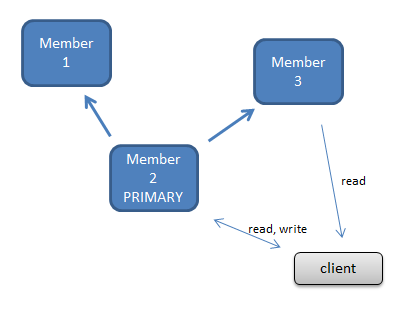
\includegraphics[]{chapters/technical-manual/replset.png}
    \end{center}
  \caption{MongoDB replica sets}\label{replica-sets}
  \end{figure}
\item[Sharding:] También conocido como particionamiento horizontal. En
  aplicaciones cuyas demandas desbordan a un único nodo, MongoDB puede
  utilizar \emph{sharding}. Básicamente consiste en particionar los
  datos por el valor de algún campo común a todos los documentos. Por
  ejemplo, en el caso de una \emph{collection}\footnote{Viene a ser
    una tabla en jerga MongoDB} conteniendo clientes se podría
  particionar por el DNI\footnote{Documento Nacional Identidad}. Así
  cada nodo tendría parte de los clientes y no todos. Como el
  particionamiento se hace manteniendo el orden es posible optimizar
  ciertas consultas de modo que solo se dirijan a un nodo. Además las
  escrituras se repartirían entre todos los nodos. Ver~\ref{sharding}
  en pág.~\pageref{sharding}.
  \begin{figure}[hbtp]
    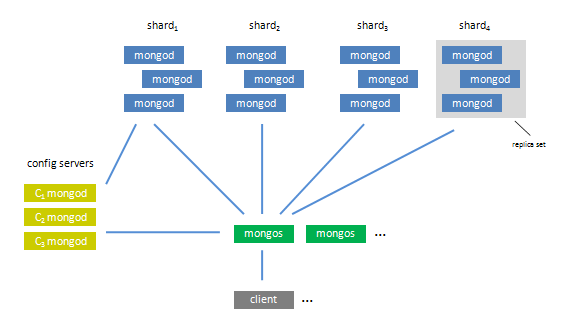
\includegraphics[width=1\textwidth]{chapters/technical-manual/sharding.png}
    \caption{MongoDB sharding}\label{sharding}
  \end{figure}
\end{description}

Vemos, pues, que MongoDB nos ofrece un buen balance de características
junto a una gran facilidad de uso. Podemos empezar a usar un único
servidor MongoDB y luego emplear \emph{replica sets} más
\emph{sharding}. Por eso, finalmente hemos elegido esta base de datos.

\subsection{DARE como procesos sin estado}

En el diseño de DARE hemos tratado de utilizar procesos sin estado y
una arquitectura en la que no se comparta el estado, \emph{shared
  nothing architecture}. Esto permite poder añadir procesos con
facilidad. También es una arquitectura más fiable, si un proceso falla
la siguiente petición puede ir a otro proceso del mismo tipo. La
escalabilidad de DARE por tanto se basa en un modelo basado en
procesos. Idealmente será responsabilidad del Sistema Operativo
relanzar los procesos que hayan terminado inesperadamente su
operación. La gran ventaja de este modelo es que para escalar
simplemente hay que lanzar más procesos ya sea en el mismo u otros
nodos.

Para ofrecer una mayor facilidad de administración los procesos Web
DARE son auto-contenidos. En vez de desplegar a un contenedor de
servlets existente, el artefacto
\emph{DARE-web<version>-standalone.jar} contiene todo lo necesario
para ejecutar un servidor web. Para ello se utiliza Jetty, que está
especialmente pensado para ser usado en modo embebido.

Hemos dicho que DARE utiliza procesos sin estado para llevar a cabo
sus actividades. Más concretamente habría dos tipos de procesos:
\begin{description}
  \item[Proceso Web:] Es fruto de ejecutar
    \emph{DARE-web<version>-standalone.jar}. Contiene Jetty, la
    aplicación web y la parte cliente de DARE-workers. Su número
    dependerá de las necesidades de escalabilidad.
  \item[Proceso Worker:] Es el fruto de ejecutar
    \emph{DARE-workers-<version>-standalone.jar}. Es responsable de
    realizar las ejecuciones de robots demandadas. Su número dependerá
    del número de ejecuciones necesarias a realizar.
\end{description}

\subsubsection{Arquitectura Backend}

En DARE llamamos \emph{Backend} a la parte responsable de almacenar
los datos y mandar las ejecuciones a aAUTOMATOR. La implementación de
esta parte se ha dividido en dos componentes: DARE-backend y
DARE-workers. Ver \ref{COMPONENTES-DARE},
pág.~\pageref{COMPONENTES-DARE}. Pero antes veamos la problemática a
afrontar y los principios por los que se guiará su implementación.

La base de datos elegida, MongoDB\ref{ELECCION-MONGO}, se encarga de
almacenar los datos. La única dificultad se presenta en convertir los
datos del dominio definidos en Java a documentos JSON y viceversa.
%TODO añadir referencia a DARE-domain

Por otro lado hay que distribuir la carga de las ejecuciones
solicitadas. Éste es un problema \emph{embarrassingly
  parallel}\cite{EMBARRASSINGLY-PARALLEL}. Cada ejecución es
completamente independiente de las otras, por lo que no hace falta
mantener una comunicación entre ellas. Esto nos permite tener un
modelo de escalabilidad muy sencillo. Simplemente hay que añadir más
threads o procesos. Finalmente nos hemos decantado por está última
opción ya que nos permite recargar la carga entre varios equipos.

El problema de utilizar procesos es que la comunicación es más
compleja. Una buena opción es utilizar el patrón
\emph{master-worker}\cite{MASTER-WORKER}. Básicamente hay procesos que
pondrían en una cola peticiones de trabajo a realizar y los
trabajadores tomarían esas peticiones de trabajo de la cola una vez
estuvieran listos. En el caso que nos ocupa hemos utilizado una ligera
variante de este patrón. En vez de introducir una nueva dependencia
usando una cola, el proceso \emph{master}\footnote{Proceso Web en este
  caso} se comunica directamente con uno de los workers. Para ello
escoge el worker que tenga una menor carga.

Aquí surge una nueva problemática: el proceso web necesita saber que
workers están disponibles. Se podrían utilizar muchas tecnologías,
pero como queríamos evitar introducir más dependencias optamos por
utilizar el sistema de almacenamiento. Así pues, cuando un worker
arranca registra su dirección IP y el puerto en el que está
escuchando. Los procesos web comprueban periódicamente que los
procesos worker gozan de buena salud y mandan las peticiones a los que
están menos ocupados.

Lo bueno de utilizar procesos sin estado es que podemos aumentar y
disminuir el número de procesos web y procesos worker según el tipo de
la carga de trabajo y la demanda del momento. La ventaja fundamental
de que sean procesos en vez de threads\footnote{hilos de ejecución} es
que podemos añadir también nuevos nodos.

\subsection{Clojure como lenguaje de programación}

Clojure es un lenguaje de programación que se ejecuta sobre la
JVM\footnote{\emph{Java Virtual Machine}}, la
CLR\cite{CLR}\footnote{\emph{Common Language Runtime}} y
JavaScript. Para este proyecto nos interesa la implementación que se
ejecuta sobre la JVM y nos referiremos a ella de ahora en adelante.

Es un lenguaje de propósito general que combina la facilidad de uso de
un lenguaje de scripting con una infraestructura robusta y eficiente
para programación concurrente. Clojure es compilado a JVM bytecode
pero aun así es completamente dinámico: cualquier característica es
soportada en tiempo de ejecución.

Clojure es un dialecto de Lisp\cite{LISP} y comparte con Lisp la
filosofía de código como datos. Ofrece, pues, un poderoso sistema de
macros. Su paradigma es eminentemente funcional ofreciendo unas
estructuras de datos inmutables y
persistentes\cite{PERSISTENT-DATA-STRUCTURES}. Cuando mutabilidad es
necesaria, Clojure ofrece memoria transaccional y un sistema de
agentes reactivos\footnote{Es similar a un Actor en Erlang}.

Clojure ofrece facilidad de acceso a librerías Java, permitiendo
reutilizar una gran cantidad de código existente. Esto le confiere ser
práctico en gran medida.

Hemos empleado Clojure en DARE-backend y DARE-workers. La razón es que
intuíamos que Clojure nos ofrecería una productividad superior. Ha
sido una experiencia muy positiva. Creemos que el código resultante es
mucho más conciso y fácil de modificar que el equivalente en Java. El
mayor problema a destacar fue la poca familiaridad con Clojure en un
primer momento.

\subsubsection{Librerías Empleadas}
\begin{description}
\item{CongoMongo}\cite{CONGO-MONGO} es un envoltorio sobre el driver
  oficial Java de MongoDB. Nos ofrece una API más adecuada para ser
  usada desde Clojure.
\item{Lamina} es una librería para trabajar con eventos como si fueran
  secuencias. Se podría decir que sigue un paradigma funcional
  reactivo\cite{FRP}. Es la base sobre la que Aleph y Gloss se
  asientan. La abstracción clave es un \emph{channel}. Combina una
  cola con el patrón publicar/subscribir.
\item{Aleph} es una librería para realizar
  I/O\footnote{Entrada/Salida} asíncrona con varios protocolos: HTTP,
  WebSockets, TCP, UDP, etc. Representa la comunicación con un
  \emph{channel} de Lamina. Aleph permite realizar una comunicación
  asíncrona de manera sencilla.
\item{Gloss} es una DSL para definir formatos de
  comunicación. Convierte un flujo de bytes en estructuras de datos
  Clojure. Esto nos facilita parsear las peticiones realizadas en vez
  de tener que trabajar con el flujo de bytes proveniente de TCP. Por
  ejemplo, para dividir el flujo de bytes en peticiones de strings se
  puede hacer definiendo un \emph{codec} en Gloss. En la
  figura~\ref{gloss-example}, pág.~\pageref{gloss-example}, se define
  que cada petición sera una String codificada en utf-8 con un entero
  indicando el tamaño de la misma.
  \begin{figure}[hb]
    \begin{center}
      \begin{lstlisting}[language=Lisp]
      (defcodec protocol-frame
        (finite-frame :int32 (string :utf-8)))
        \end{lstlisting}
    \end{center}
  \caption{Ejemplo uso Gloss}\label{gloss-example}
  \end{figure}
\end{description}

\subsection{Librería para Python}

Hemos decidido hacer una librería para Python aparte de una en
Java. La idea es poder ofrecer una alternativa más sencilla que
Java. Python nos permite que el programador tenga un ejemplo
funcionando en menor tiempo. Además sus tiempos de arranque son
pequeños, lo que nos permite que sea la base para crear una aplicación
de línea de comandos.

Python es un lenguaje muy legible. Soporta varios paradigmas,
imperativo, OOP\footnote{\emph{Object Oriented Programming}}, y
funcional. Además cuenta con numerosas librerías de gran calidad lo
que siempre lo hace una opción interesante.

Una duda que nos asaltó fue si utilizar la versión 3 de Python. Es la
última versión del lenguaje y cuenta con ciertas mejoras pero su
presencia no es tan ubicua. Finalmente este último aspecto nos ha
decantado a favor de Python 2.

\subsubsection{httplib2}

Para realizar la librería hemos empleado httplib2. Esta librería
cliente HTTP nos ofrece ventajas con respecto a las librerías
incluidas por defecto en la distribución de Python. Las librerías
incluidas httplib y urllib son de nivel más bajo. Tendríamos, por
ejemplo, que manejar ciertos aspectos de HTTP como caching
manualmente.

Más concretamente httplib2 nos ofrece:
\begin{description}
  \item[Soporte Keep-Alive]: Permite mantener el mismo socket abierto
    y reutilizarlo para hacer varias peticiones.
  \item[Soporte Autenticación]: Soporta varios tipos de
    autenticación HTTP como Digest, Basic y WSSE.
  \item[Soporte cacheado]: Tiene una caché privada que se conserva
    entre requests. Entiende la cabecera Cache-Control y los
    validadores ETag y Last-Modified.
  \item[Soporte métodos HTTP]: Soporta todos los métodos HTTP, no solo
    GET y POST.
  \item[Soporte Redirects]: Procesa automáticamente los redirects
    devueltos por el servidor web.
  \item[Soporte Comprensión]: Puede recibir respuestas comprimidas ya
    sea con comprensión deflate o gzip.
\end{description}

\subsection{Interfaz Línea Comandos en Python}

La idea es poder ofrecer una aplicación que permita emplear DARE de
una manera sencilla y directa. Además nos permitía probar la librería
en un caso de uso real. Hemos empleado la librería en Python DARE para
realizarla. Python dispone además de librerías muy completas para el
manejo y parseado de argumentos como argparse. Por brevedad, nos
referiremos de ahora en adelante a esta aplicación \emph{dare.py}.

Una característica que queríamos añadir a esta aplicación es la
posibilidad de recordar los robots y los resultados que has tenido
anteriormente. Creemos que esto facilitaría en gran medida el trabajo
al usuario, podría ver los robos que ha creado y los resultados
obtenidos. Para ello necesitamos un sistema de almacenamiento que
conserve esos datos entre diferentes invocaciones a \emph{dare.py}.

\subsubsection{SQLite}

Para realizar esta labor de almacenamiento nos hemos decantado por
SQLite\cite{SQLite}. SQLite nos ofrece una base de datos relacional en
la forma de una librería de tamaño reducido, permitiéndonos usarla en
modo embebido. Es muy fácil de usar, no requiere configuración para
empezar a ser usada y su rendimiento es de sobra adecuado para nuestra
necesidad concreta.

Es muy usada como sistema de almacenamiento local, justo el caso que
nos ocupa.

\subsection{Componentes}
\label{COMPONENTES-DARE}
A continuación veamos una visión general del proyecto desde el punto
de vista de un diagrama de componentes UML. En el se muestran los
componentes presentes y las relaciones entre los mismos. A mayores
vamos a realizar una breve descripción de cada uno de ellos:

\begin{description}

\item[minilenguaje:] Es el componente que implementa la DSL definida
  por el proyecto. Este lenguaje se ha denominado minilenguaje. Es
  responsable de transformar la DSL en el formato XML entendido por
  \emph{aAUTOMATOR Runtime}\footnote{Está contenido dentro del
    artefacto \emph{StringEditor}}. Está implementado en JRuby y
  Java. La parte en JRuby se encarga de definir una DSL interna y la
  parte Java ofrece una API a la misma.
\item[DARE-domain:] Define un modelo de dominio del sistema. Facilita
  una comprensión conceptual del sistema, abstrayéndonos de otras
  consideraciones. Contiene clases como Robot, ExecutionResult y
  PeriodicalExecution. Instancias de estas clases son creadas cuando
  se obtienen datos del sistema de almacenamiento. Está implementado
  en Java.
\item[DARE-war:] Es una aplicación web Java. Contiene todos los
  componentes dentro del recuadro servicio. Puede ser desplegado en
  cualquier servidor de aplicaciones JEE y/o contenedor de servlets.

  Siguiendo el patrón MVC\footnote{Modelo Vista Controlador} este
  modelo es el responsable de la parte de vista y controlador. Utiliza
  la API JAX-RS para lleva a cabo esta labor. Utiliza a DARE-domain
  como modelo y DARE-backend ofrecería servicios de persistencia y
  ejecución.

  Este componente ha sido concebido de modo que se puede desplegar en
  varios nodos, ya que se sigue una filosofía
  \emph{share-nothing}. Para ellos nos hacemos valer de las
  características sin estado de REST. Es decir, podemos tener varios
  servidores web ejecutándose en distintos nodos. Está implementado en
  Java.

\item[DARE-backend:] Es el componente encargado de comunicarse con la
  base de datos MongoDB tanto para leer como para escribir los objetos
  definidos en DARE-domain. Recibe también las peticiones de ejecución
  para aAUTOMATOR. Luego utilizando la parte cliente de DARE-workers
  las reparte entre los procesos \emph{worker} que se están
  ejecutando. Está implementado en Clojure.

\item[DARE-workers:] Este componente está compuesto por una parte
  cliente que lanza peticiones de ejecución a aAUTOMATOR. La parte
  servidor, de ahora en adelante \emph{worker}, interpreta esas
  peticiones y hace el trabajo correspondiente. Uno o varios de estos
  workers pueden estar lanzados en función de las necesidades de
  escalabilidad y fiabilidad necesarios.

  Cada worker es un proceso por lo que alguno de ellos podría dejar de
  funcionar y DARE podría seguir ofreciendo su servicio. Además al ser
  cada uno un proceso se pueden ejecutar localmente en el mismo nodo o
  repartirlo a través de varios nodos del cluster. La parte cliente es
  capaz de descubrirlos y repartir la carga de peticiones entre los
  workers. Aparte comprueba continuamente el estado de salud de los
  workers para que el servicio continúe funcionando aun en la
  presencia de errores en los workers.

 Tanto la parte servidor como cliente están implementados en Clojure.

\item[DARE-util:] Es un cajón de sastre donde se encuentran diversas
  funciones de utilidad usadas por varios otros módulos.

\item[DARE-web:] Este módulo se utiliza para facilitar el despliegue
  de la aplicación. Toma el fichero \emph{war} con la aplicación y lo
  ejecuta creando un servicio web. Para ello emplea el contenedor de
  servlets embebido, Jetty\cite{JETTY}. Jetty es un contenedor de
  servlets ligero, por lo que es especialmente adecuado para lanzar
  numerosas instancias de la aplicación. Este componente está
  implementado en Clojure.

\item[DARE-java:] %TODO extract
\item[DARE-python:] Este módulo implemente la librería cliente para
  Python, así como la aplicación de línea de comandos. Como se ha
  descrito anteriormente usa httplib2 para llevar a cabo la
  comunicación con el servicio.

  La aplicación de línea de comandos está contenida en este componente
  y utiliza la librería creada para llevar a cabo su
  funcionalidad. Como es lógico está implementado en Python.
\end{description}

\begin{landscape}
\begin{figure}[p]
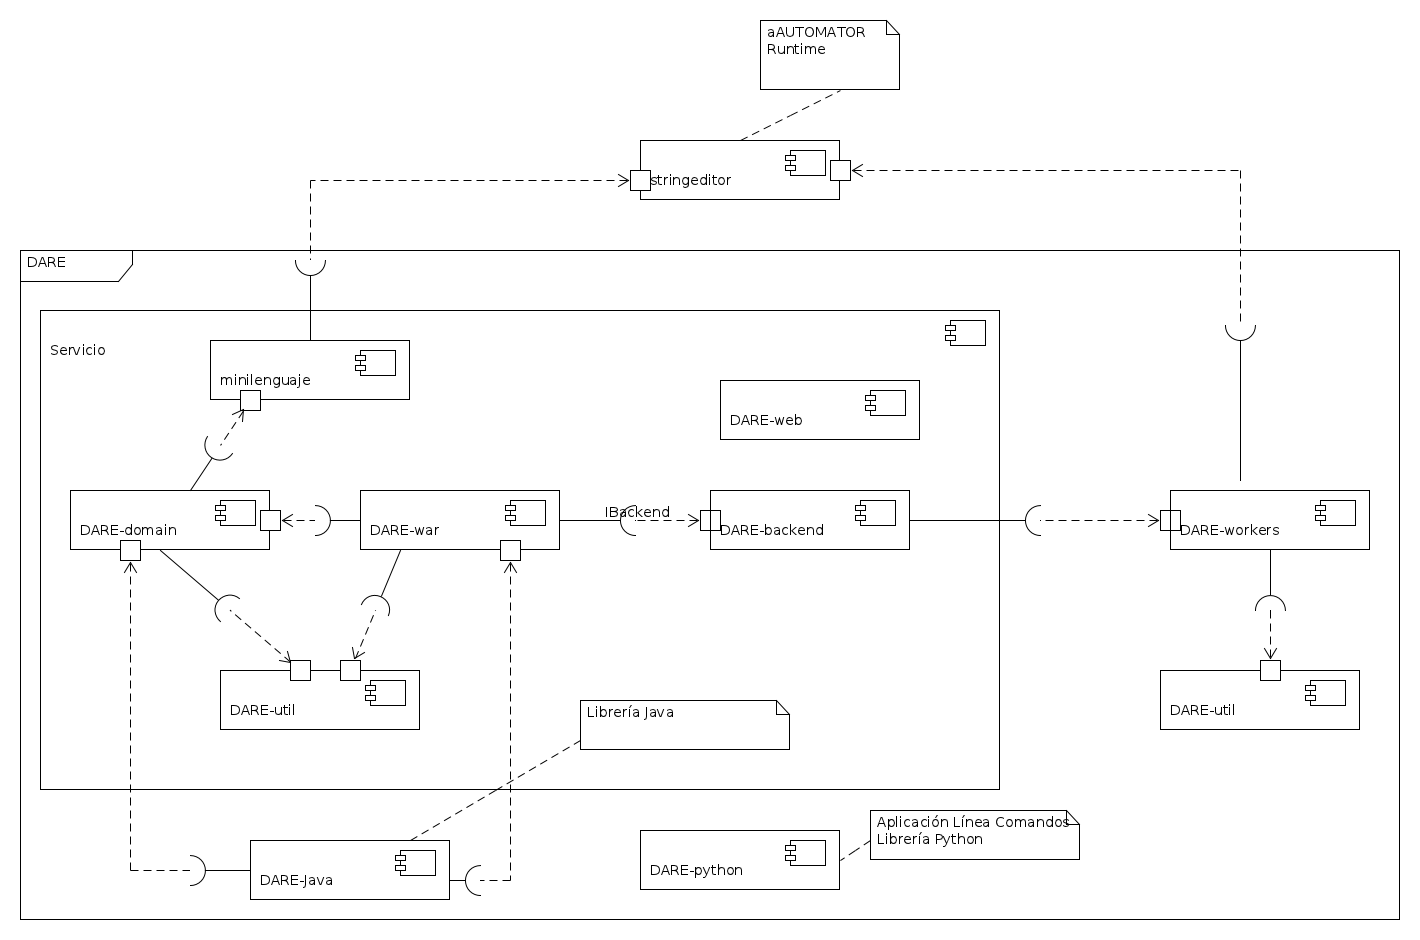
\includegraphics[width=1.4\textwidth]{chapters/technical-manual/diagrams/diagrama_componentes.png}
\caption{Diagrama Componentes DARE}\label{diagrama_componentes_dare}
\end{figure}
\end{landscape}

\subsubsection{Diagrama clases minilenguaje}

En este diagrama mostramos las clases con las que se implementa la DSL
interna propuesta.

Por un lado tenemos la clase \emph{Transformer}. Un objeto de esta
clase se corresponde a uno de los transformadores de los que está
compuesto un robot. Ver~\ref{COMPORTAMIENTO_AUTOMATOR},
pág.~\pageref{COMPORTAMIENTO_AUTOMATOR}. Sigue el patrón
Composite\cite{COMPOSITE_PATTERN}, es decir, cada \emph{Transformer}
puede a su vez tener \emph{Transformers} hijos. Cada
\emph{Transformer} es capaz de convertirse al XML que necesita
aAUTOMATOR. Cada subclase de \emph{Transformer} se corresponde a una
clase \emph{Transformer} de aAUTOMATOR. Cada \emph{Transformer} va a
necesitar una serie de parámetros requeridos y opcionales. Cada
subclase de \emph{Transformer} define pues, los parametros que va a
necesitar de una manera declarativa. \emph{Transformer} mantiene una
lista de los hijos que contiene y permite que se le añadan más. Además
puede recibir un XML de aAUTOMATOR y convertirlo a una \emph{string}
de minilenguaje que produciría ese XML.

La clase \emph{Language} es la encargada de procesar el
lenguaje. Basicamente el lenguaje se evalúa contra una instancia de
\emph{Language}. Por ejemplo, el minilenguaje definido por
\emph{xpath('//a/@href')} implica que el método xpath de
\emph{Language} es llamado. ¿Implica ésto que habría que definir
métodos por cada \emph{Transformer} que se defina? No, empleando
metaprogramación\cite{METAPROGRAMMING} cada vez que se define una
subclase de \emph{Transformer} se crea dinámicamente un nuevo método
en \emph{Language}. Llamar a este método implica crear el
\emph{Transformer} de la subclase adecuada con los parámetros
indicados. En este momento el \emph{Transformer} creado se añade al
que está ligado al de \emph{Language}. Es decir, según se van llamando
a los métodos que crean los transformers estos se van añadiendo al
transformer de primer nivel en el \emph{Language}. Por ejemplo,
\emph{url | xpath('//a/@href') | patternMatcher('(http://.*)')} añade
tres \emph{Transformers} al \emph{Transformer} padre, que por defecto
está en modo cascade. Como se puede ver se emplea el operador \emph{|}
para separar cada \emph{Transformer}. Esto no es más que azúcar
sintático. El siguiente ejemplo sería equivalente: \emph{url;
  xpath('//a/@href'); patternMatcher('(http://.*)')}, pero con el
operador \emph{|} queda más clara la intención.

\emph{Language} tiene los métodos \emph{pipe} y \emph{branch}. Estos
métodos definen un nuevo \emph{Transformer} con semánticas de CASCADE
o de BRANCH. Por tanto, para \emph{branch} se requiere indicar el
BRANCH~TYPE y el MERGE~MODE. Estas llamadas crear un nuevo
\emph{Language} con su correspondiente \emph{Transformer}. Estos
métodos reciben un bloque de código que se interpretará en el contexto
de la nueva instancia de \emph{Language}.

\emph{DocumentWrapper} y \emph{AttributesWrapper} se encargan de
facilitar la generación del XML.

\begin{landscape}
\begin{figure}[hp]
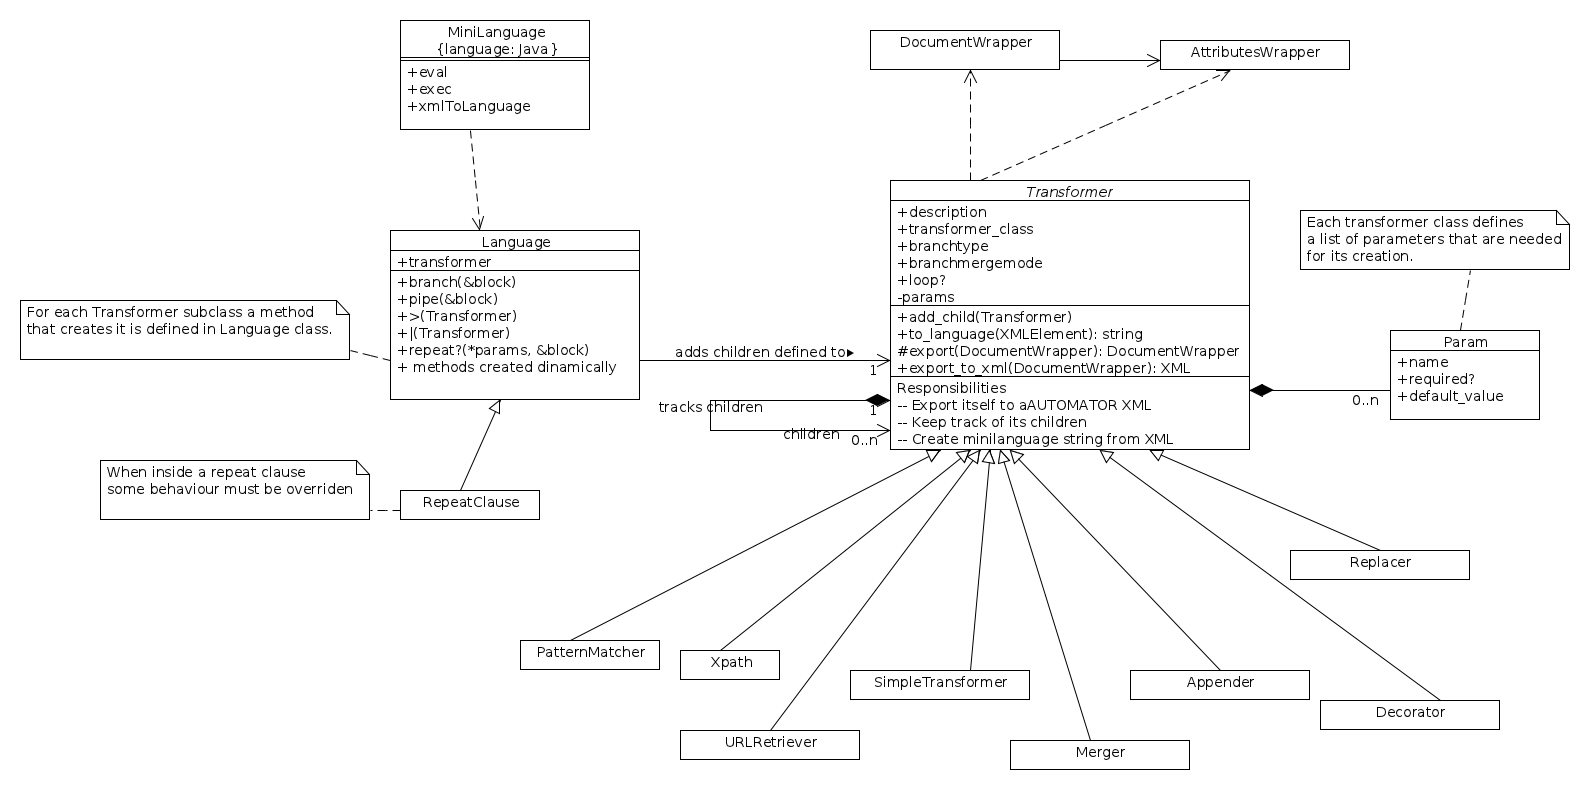
\includegraphics[width=1.4\textwidth]{chapters/technical-manual/diagrams/clases_minilenguaje.png}
\caption{Diagrama clases Minilenguaje}\label{diagrama_clases_minilenguaje}
\end{figure}
\end{landscape}

\subsubsection{Descripción Implementación transformer.rb}
Descripción general \ldots{}
% transformer.rb en modo literario

\subsubsection{Diagrama clases DARE-domain}

En el diagrama de clases de entidades,
\ref{diagrama_clases_entidades_domain}
pág.~\pageref{diagrama_clases_entidades_domain}, se muestran las
entidades por las que está formada la aplicación. Por cada
\emph{Robot} puede haber cero, uno o varios
\emph{ExecutionResult}. Por cada \emph{ExecutionResult} hay un
\emph{Robot}. Por cada \emph{Robot} puede haber cero, uno o varios
\emph{PeriodicalExecution}. Por cada \emph{PeriodicalExecution} hay un
\emph{Robot}. Una \emph{PeriodicalExecution} no contiene un
\emph{ExecutionResult} si todavía no se ha completado la
ejecución. Una vez se ha completao el \emph{PeriodicalExecution}
contiene el \emph{ExecutionResult} de su última ejecución.

\emph{Robot} llama a MiniLanguage para generar el XML de aAUTOMATOR a
partir del minilenguaje que haya sido creado. Contiene métodos para
crear tanto un nuevo \emph{ExecutionResult} como una nueva
\emph{PeriodicalExecution}. Un \emph{Robot} no contiene directamente
las \emph{PeriodicalExecution} y los \emph{ExecutionResult}
asociados. Las asociaciones solo indican la cardinalidad existente. El
\emph{ExecutionResult} no contiene una referencia al \emph{Robot}
asociado, solo guardan el código del \emph{Robot}
asociado. \emph{PeriodicalExecution} si que contiene su
\emph{ExecutionResult} asociada.

Por lo demás DARE-Domain define una serie de interfaces y clases de
utilidad usadas por DARE-war. La interfaz clave es \emph{IBackend}. La
implementación de esta interfaz debe ser capaz de eliminar y guardar
las entidades definidas por DARE-Domain. Se definen dos excepciones
que se pueden producir relacionadas con el manejo de
ejecuciones. \emph{IBackendBuilder} define una interfaz para el objeto
que debe de crear el \emph{IBackend} a ser usado. Define y acepta una
serie de parámetros necesarios para la operativa concreta del backend
selecionado.

La clase \emph{Maybe} sirve para indicar que un resultado es
opcional. Por otra parte \emph{MinilanguageProducer} sirve para mantener una
lista de instancias de \emph{Minilanguage} preparadas para ser
usadas. Ver~\ref{interpreter_state_manipulation},
pág.~\pageref{interpreter_state_manipulation}.

\begin{landscape}

\begin{figure}[hp]
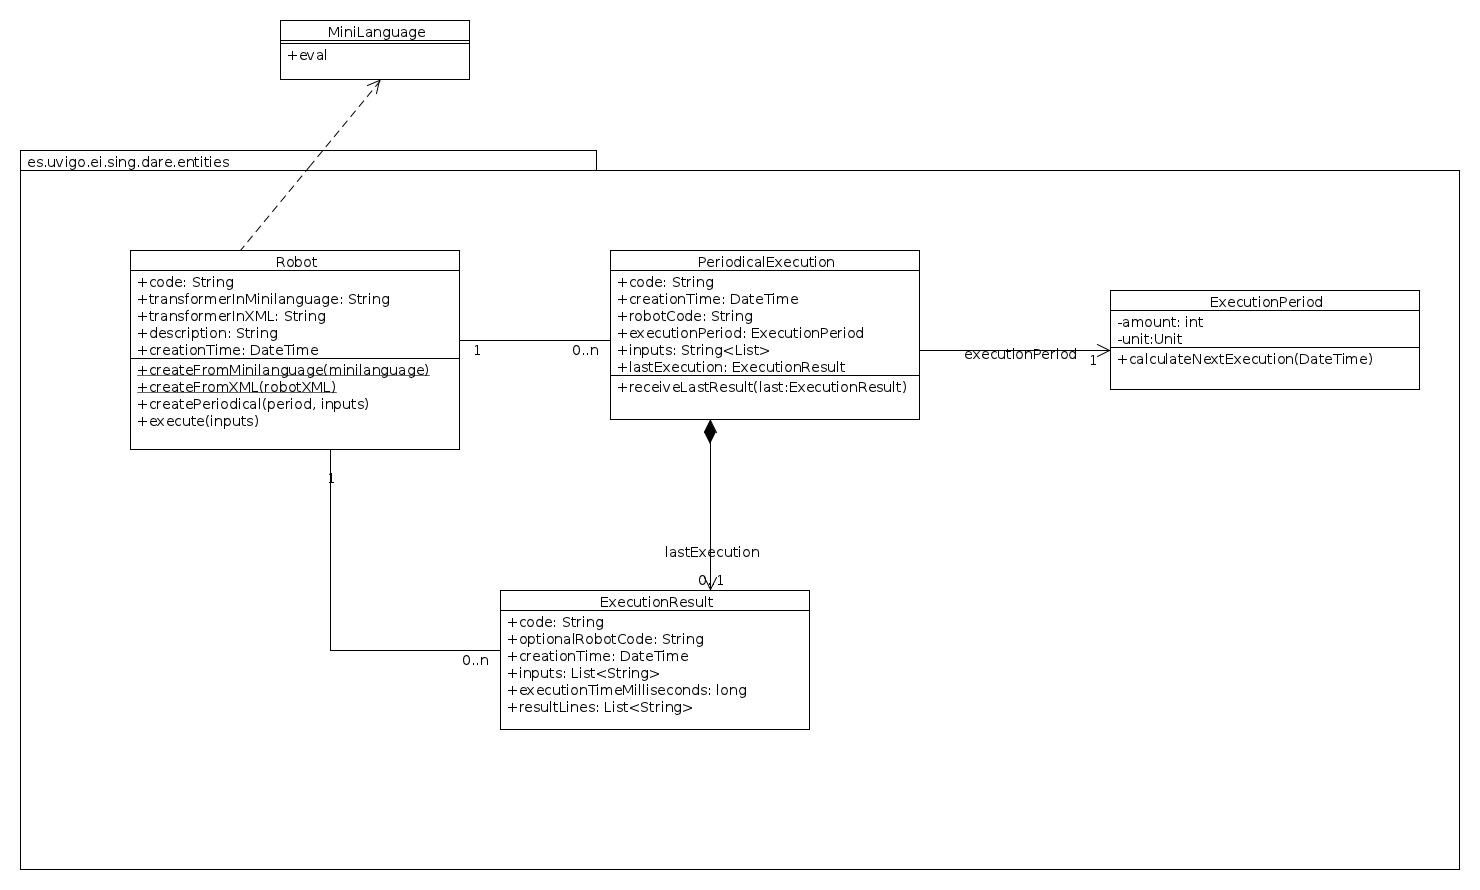
\includegraphics[width=1.4\textwidth]{chapters/technical-manual/diagrams/entidades_domain.png}
\caption{Diagrama clases detallado de Entidades}\label{diagrama_clases_entidades_domain}
\end{figure}

\begin{figure}[hp]
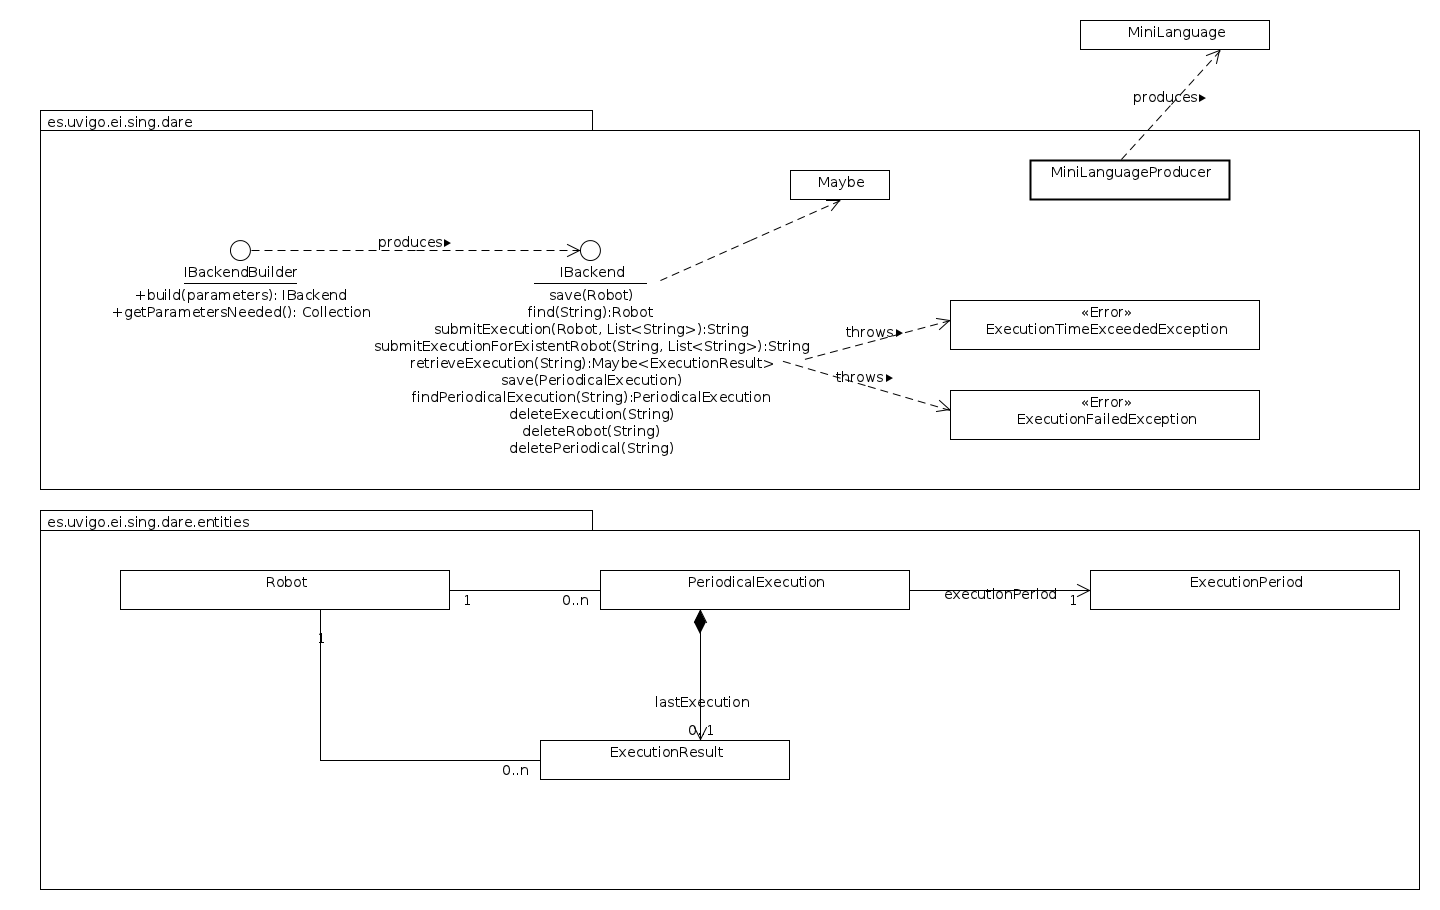
\includegraphics[width=1.4\textwidth]{chapters/technical-manual/diagrams/clases_domain.png}
\caption{Diagrama clases Domain}\label{diagrama_clases_domain}
\end{figure}

\end{landscape}

\subsubsection{Diagrama clases DARE-war}

Se muestran las clases de este componente agrupadas en paquetes junto
a clases de otros componentes que son de interés.

\emph{ConfigurationBootstrapper} es una clase que a partir del
contexto web crea un objeto \emph{Configuration}. Este objeto se
guarda en el contexto de la aplicación web y está disponible para los
recursos. El objeto \emph{Configuration} tiene referencias a la
implementación de \emph{IBackend} que se va a usar y el
\emph{MinilanguageProducer}.

En el paquete resources están definidas varias clases que definirán
los recursos REST de los que se compone la aplicación web. Vienen a
cumplir la función de controladores y utilizan la librería
JAX-RS. Estos controladores utilizan \emph{IBackend} para guardar y
obtener las entidades. Además le piden a \emph{IBackend} que se
realicen ejecuciones. Como resultados de algunas operaciones de
lectura se crean objetos del paquete views.

En el paquete views están definidos varios objetos con escasa lógica
que definen estructuras de datos que se van a traducir a XML y
JSON. La estructura de estas clases y del JSON o XML generado es la
misma. Para hacer la traducción JAX-RS utiliza JAXB\cite{JAXB}.

\begin{landscape}
\begin{figure}[hp]
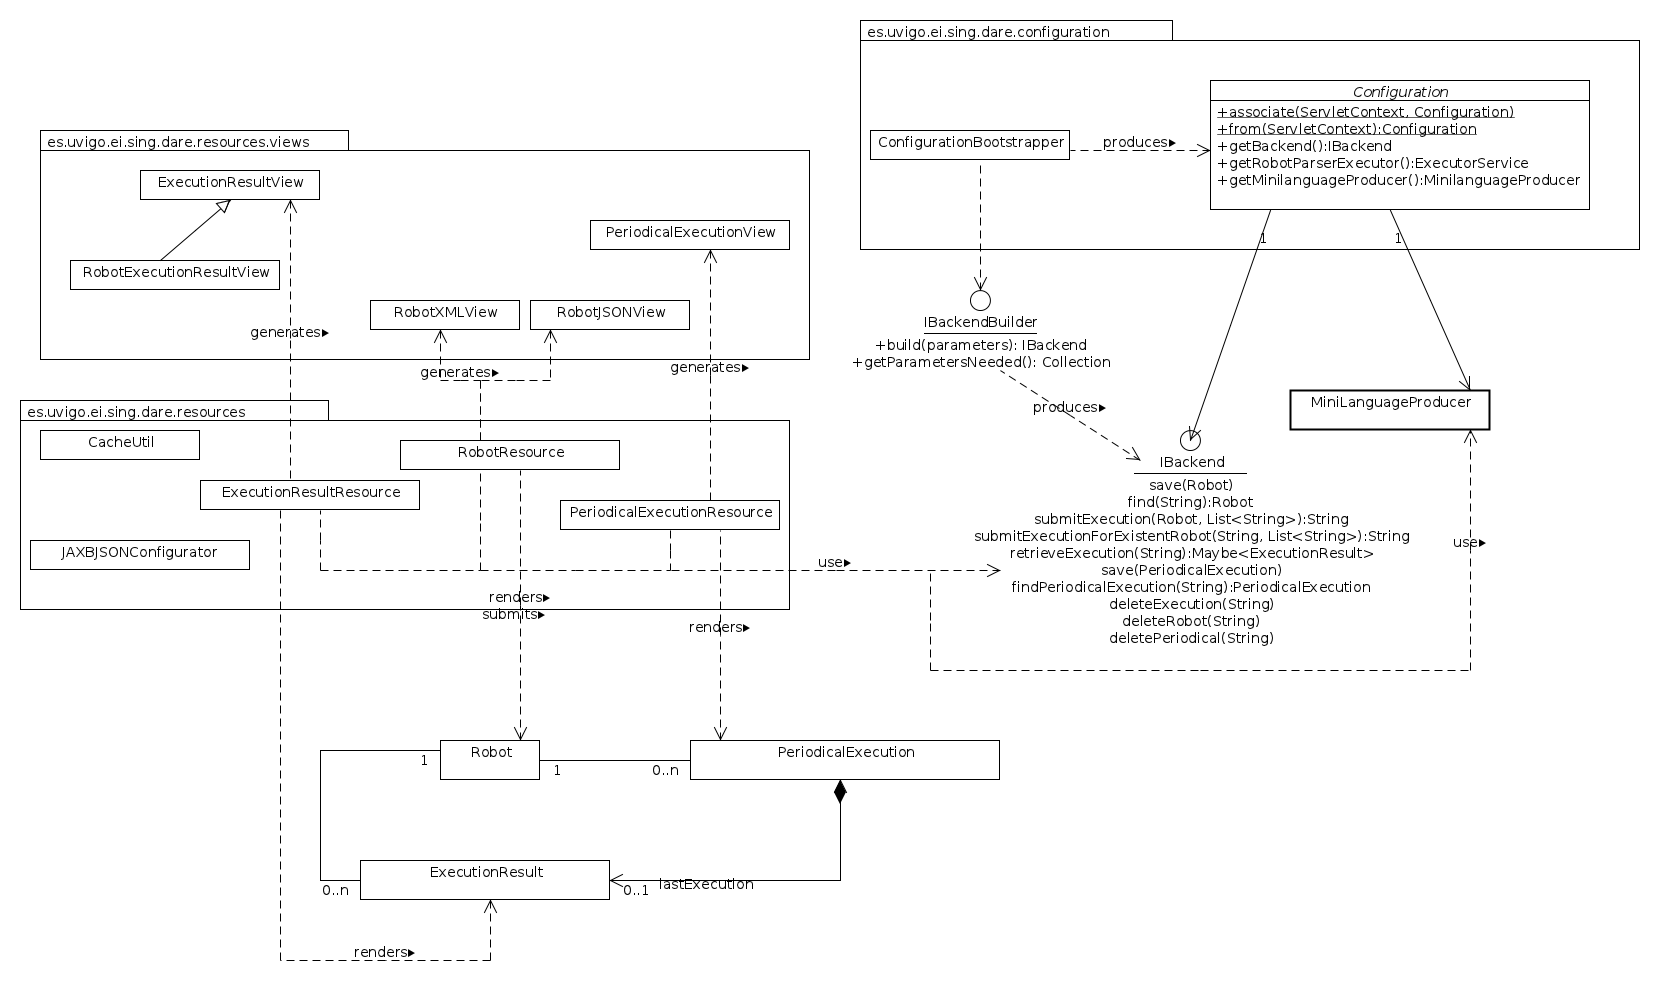
\includegraphics[width=1.4\textwidth]{chapters/technical-manual/diagrams/clases_war.png}
\caption{Diagrama clases WAR}\label{diagrama_clases_war}
\end{figure}
\end{landscape}

\subsubsection{Diagrama clases DARE-backend}
% a fondo backend/core.clj?
\subsubsection{Diagrama clases DARE-workers}
% a fondo workers/client.clj, workers/server.clj?

\subsubsection{Esquema datos Sistema Almacenamiento}
